% Chapter 11

\chapter{Correction factors to the multiplicities} % Chapter title

\label{ch:CF} % For referencing the chapter elsewhere, use \autoref{ch:name}

%----------------------------------------------------------------------------------------

The \textit{raw} charged multiplicities presented in the previous chapter need to be corrected. The corrections discussed here are the acceptance correction i.e. the correction due to the geometrical limitation of the spectrometer and the data reconstruction efficiency as well as the diffractive vector meson correction and the radiative correction. the electron contamination correction, which is included in the acceptance correction,

\section{Determination of the spectrometer acceptance} \label{sec:Acc}

\subsection{Monte Carlo sample from DJANGOH}

The COMPASS detector does not cover the full phase-space, thus the measured multiplicities have
to be corrected for the finite detector acceptance, which is of the order of $70$\%. The correction is
done using a Monte-Carlo dataset containing about $400$ million events generated in the kinematic
region $Q^2 > 0.8$ (GeV/$c$)$^2$, $x$ $\in$ [$10^{-4},0.9$], $y$ $\in$ [$0.01,0.95$], thanks to the Blue Waters facility computing power \cite{Bode2013,Kramer2015}. The kinematic region is larger than the one of interest in the analysis. This is done in order to be able to take into account bin-to-bin migration of events. Two different MC samples with a different beam charge are providing $200$ millions events in total to take into account any asymmetry in the spectrometer relative to the beam charge. As there is a difference of two slabs in the OT in the experimental setup between the periods P$07$ and P$08$ onwards, two different acceptance corrections should be applied. The two different MC samples were both reconstructed twice. One reconstruction is done without the two inefficient OT slabs and will give P$07$ acceptance while the other is done with all the slabs and will give P$08^+$ (P08 and following periods) acceptances. Eventually from two samples, four different acceptances are computed (P$07$-$\mu^+$, P$07$-$\mu^-$, P$08^+$-$\mu^+$ and P$08^+$-$\mu^+$).

The events are generated with the DJANGOH generator with a parametrization of the parton distribution functions (MSTW08 \cite{MSTW08}). In addition, the use of JETSET inside DJANGOH allows the hadronization of quarks q to final-state hadrons h according to the Lund model. The COMPASS high $p_T$ tuning was used for the JETSET parameters. The events of DJANGOH are then propagated into the experimental setup simulated by TGEANT. The beam and beam reconstruction is not simulated but the reconstructed beam tracks from data are being used. The output of this chain is referred to as \textit{generated} sample. These events are then reconstructed with the same CORAL code as used to reconstruct real data. This new sample is called \textit{reconstructed} sample. The same DIS event and unidentified hadron selection that are used on real data (except cuts related to beam and beam reconstruction) are applied to the MC data sample for reconstructed MC events and particles.

The acceptance is calculated as the ratio of reconstructed over generated particles. In both cases, the particle ID is taken from the MC truth. The following selection is made on the generated particles:

\begin{enumerate}
  \item Energy of the beam muon in range [140,180] GeV
	\item Z coordinate of event vertex ($z_{vtx}$) within the target region $\in$ [-325 cm, -71 cm]
	\item Primary interaction in the target material (PHAST routine PaAlgo:InTarget() for both data and MC (Section \ref{sec:targetcut}) target positions to have a complete overlap of coverage)
	\item Beam track crossing the entire target (PHAST routine PaAlgo:CrossCells())
  \item $Q^2>1$ (GeV/c)$^2$
  \item $0.1 < y < 0.7$
	\item $5$ GeV/$c^2$ $< W < 17$ GeV/$c^2$
  \item $0.004 < x < 0.4$
  \item $\nu$ range used in data
  \item $0.2 < z < 0.85$
\end{enumerate}

The inclusive kinematic variables $Q^2$, $x$ and $y$ and semi-inclusive variables $z$ and $p_h$ are shown in Figs.~\ref{pic:MCDISkin} and~\ref{pic:MCSIDISkin} for real data (red) and reconstructed MC data (blue). The ratio between real data and reconstructed MC data is shown at the bottom of each panel. A relative good agreement is reached, except in the low statistics high $x$ and high $Q^2$ regions and for $\theta_h$. It was shown in previous work that the COMPASS acceptance nearly factorizes in $A_{muon} \cdot A_{hadron}$. Thus for multiplicities $A_{muon}$ drops out in a large extent and the difference of data and MC in edges of the muon kinematics does not introduce a bias. The description of $\theta_h$ should be improved.

\begin{figure}[!h]
  \centering
	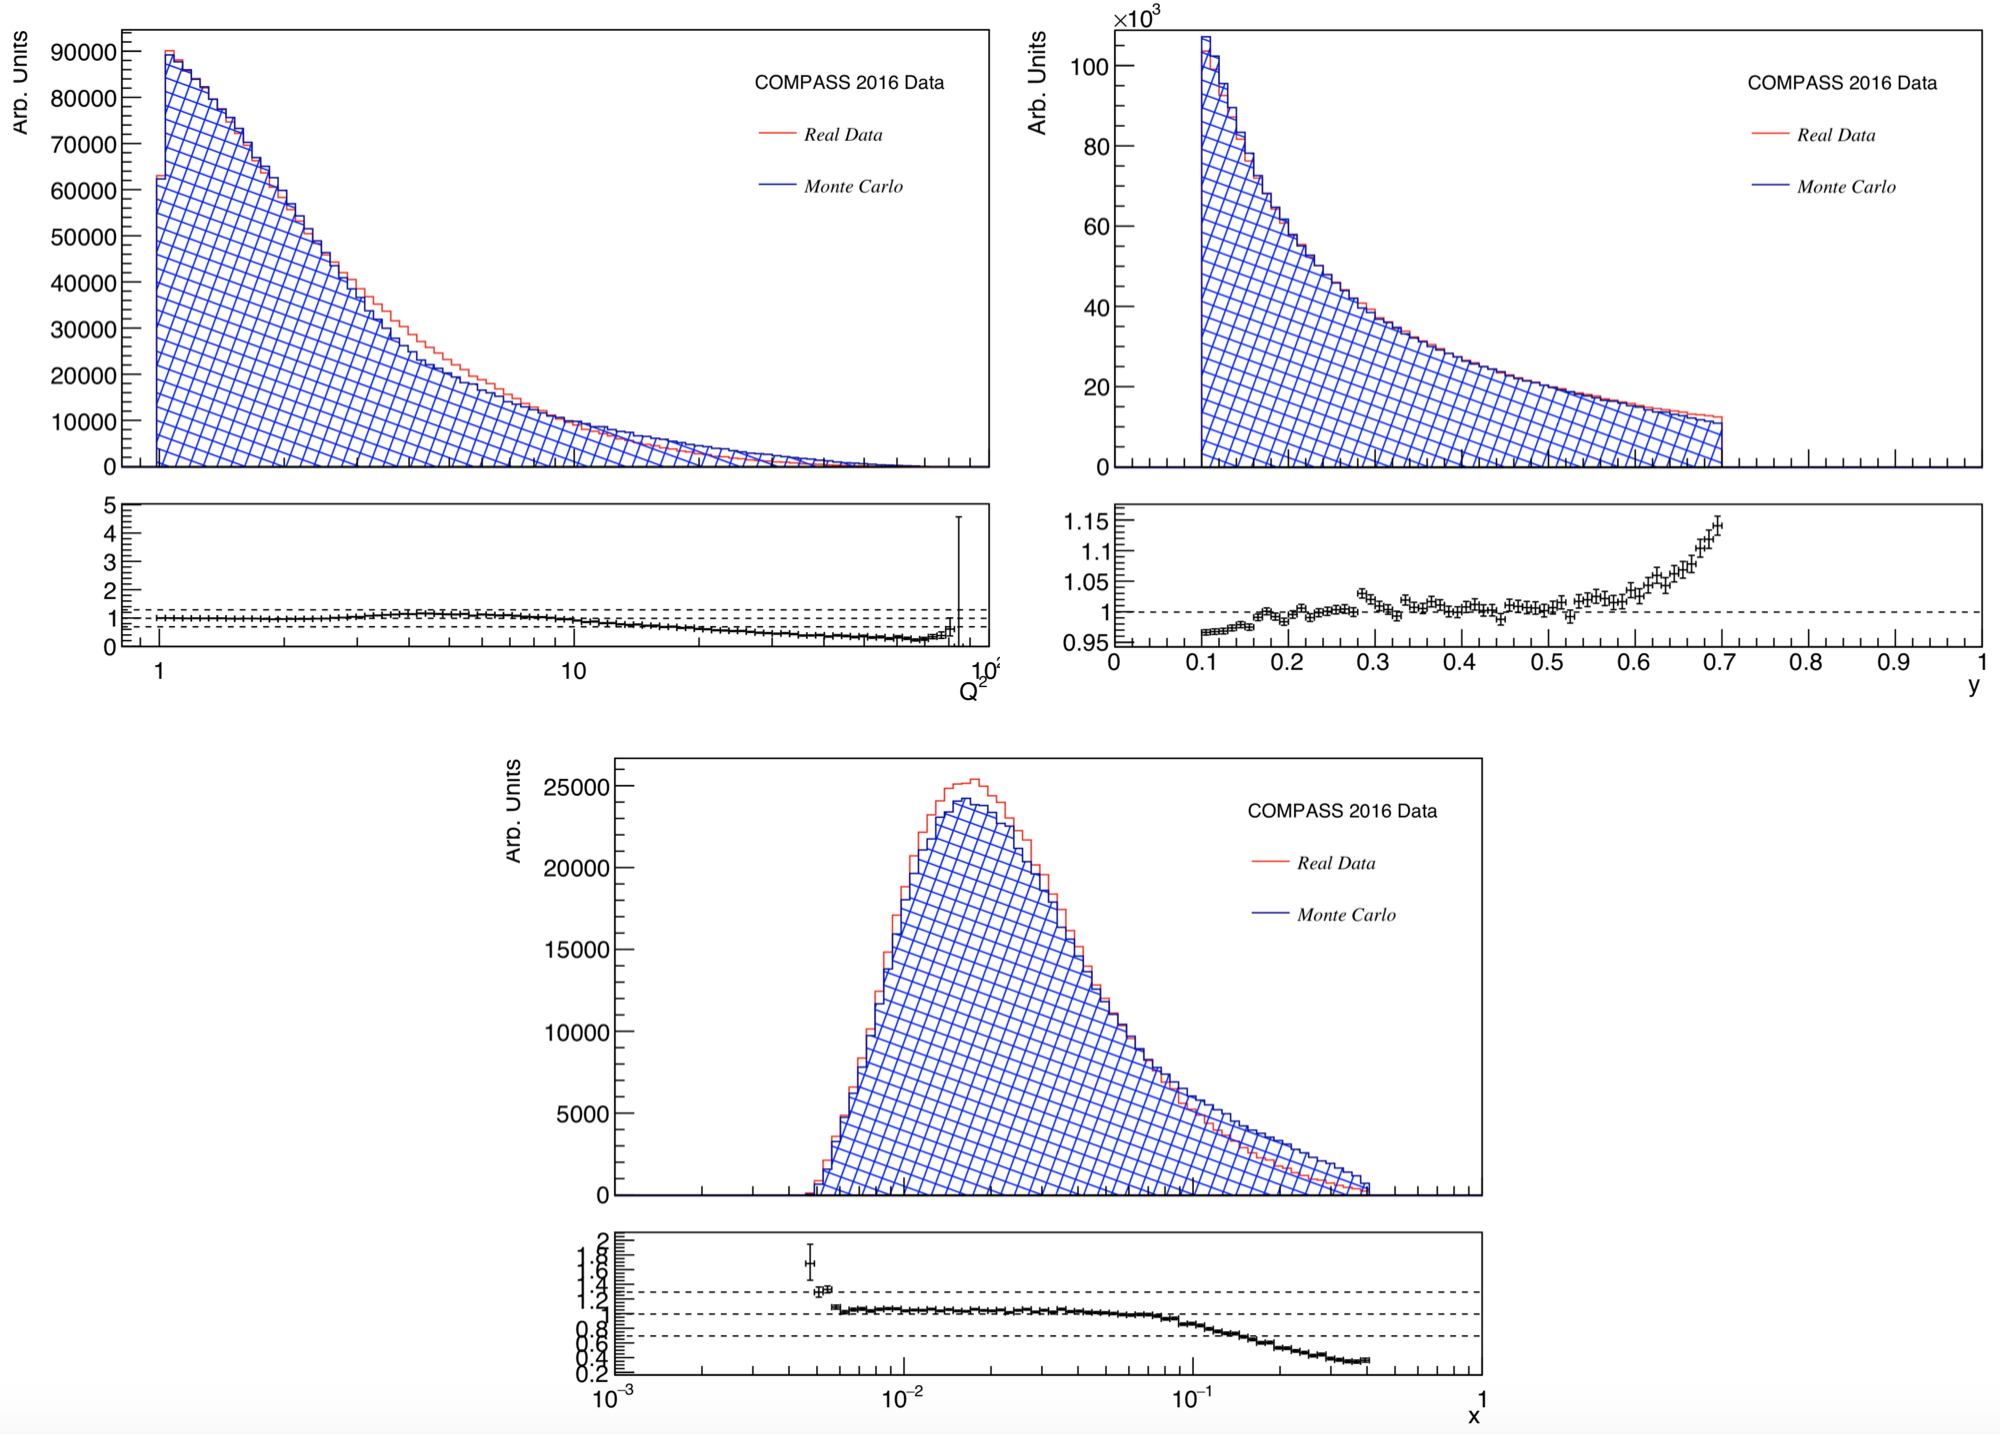
\includegraphics[scale=0.50]{./gfx/DIS_kin.png}
	\caption{Kinematical variables for DIS events ($Q^2$, $y$ and $x$) for Data (red) and Monte-Carlo (blue), as well as the ratio Data/Monte-Carlo.}
	\label{pic:MCDISkin}
\end{figure}

\begin{figure}[!h]
  \centering
	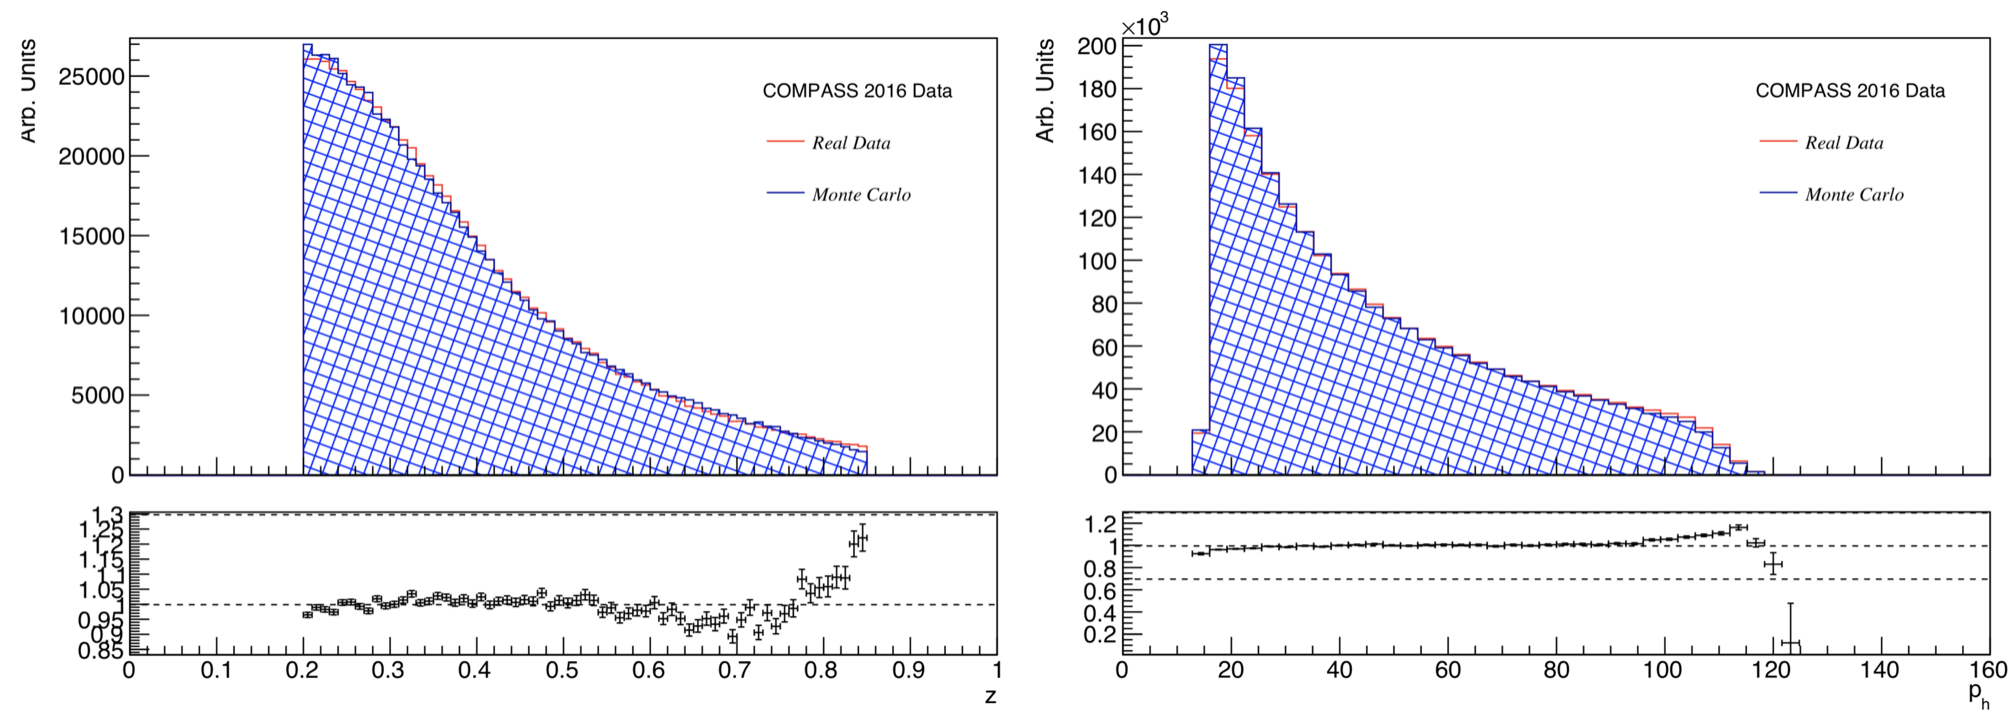
\includegraphics[scale=0.50]{./gfx/SIDIS_kin.png}
	\caption{Kinematical variables for charged hadrons ($z$, $p_h$ and $\theta_h$) for Data (red) and Monte-Carlo (blue), as well as the ratio Data/Monte-Carlo.}
	\label{pic:MCSIDISkin}
\end{figure}

\subsection{Acceptance calculation}

In the following, $r$ and $g$ refers to 'reconstructed' and 'generated' quantities.

The acceptance is determined as the ratio of reconstructed multiplicities $M^h_r$ over the generated multiplicities $M^h_g$ and is binned as for the data in $x$, $y$ and $z$:

\begin{equation}
  A^h(x,y,z) = \frac{M^h_r(x_r,y_r,z_r)}{M^h_g(x_g,y_g,z_g)}=\frac{N^h_r(x_r,y_r,z_r)/N^{DIS}_r(x_r,y_r,z_r)}{N^h_g(x_g,y_g,z_g)/N^{DIS}_g(x_g,y_g,z_g)}
\end{equation}

where $x_g$, $y_g$ and $z_g$ are the generated kinematic values and $x_r$, $y_r$ and $z_r$ are the reconstructed kinematic values. The acceptance being calculated in this fashion, the kinematic bin migration due to reconstruction limitations is accounted for. A more rigorous bin migration correction would involve an unfolding procedure but is not done in this analysis.

For this method, the error estimation is difficult to rigorously calculate as the numbers of evaluated hadrons and DIS events, in both the reconstructed and generated case, are not independent. In the following, all quantities are binned in ($x,y,z$). An estimate is made by assuming on the basis that there are much more DIS events than hadrons. Due to the $z$ kinematic bin migration effects, there exist particles in $N_r$, which does not belong to $N_g$. Decomposing $N_r$ into two contributions namely $N_{r^0}$, which are contained in $N_g$ and $N_{r'}$, which are not, the final acceptance error yields:
%
\begin{equation}
  \begin{split}
    E^2_{acc} = \left (\frac{G_D}{R_D+R'_{D}}\right )^2\left [\frac{(R_h+A)(G_h-R_h+1)}{(G_h+2)^2(G_h+3)}+\frac{R'_{h}}{G^2_h}+\frac{R'^2_h}{G^3_h}\right ] \\
                + \left (\frac{G_D}{R_D+R'_{D}}\right )^4\left (\frac{R_h+R'_h}{G_h}\right )^2\left [\frac{(R_D+1)(G_D-R_D+1)}{(G_D+2)^2(G_D+3)}+\frac{R'_D}{G^2_D}+\frac{R'^2_D}{G^3_D}\right ],
  \end{split}
\end{equation}
%
where $G_h$ ($G_D$) are the generated hadrons (DIS events) in a given $x$, $y$, $z$ bin, $R_h$ ($R_D$) the reconstructed hadrons (DIS events) and $R'_h$ ($R'_D$) all other particles (events) that are reconstructed as hadrons (DIS events) in a given $x$, $y$, $z$ bin.

The acceptance correction factors $A^h(x,y,z)$ for unidentified hadrons, pions, kaons and protons are shown in Figs.~\ref{pic:AccH} to \ref{pic:AccP} for the P$07$ sample. The acceptance results are displayed versus $z$ and each pad is a ($x,y$) bin, left to right for increasing $x$ and top to bottom for increasing $y$. Note that the acceptance is very similar for positive and negative particles and for $\mu^+$ and $\mu^-$ beams.

\begin{sidewaysfigure}[!]
  \centering
	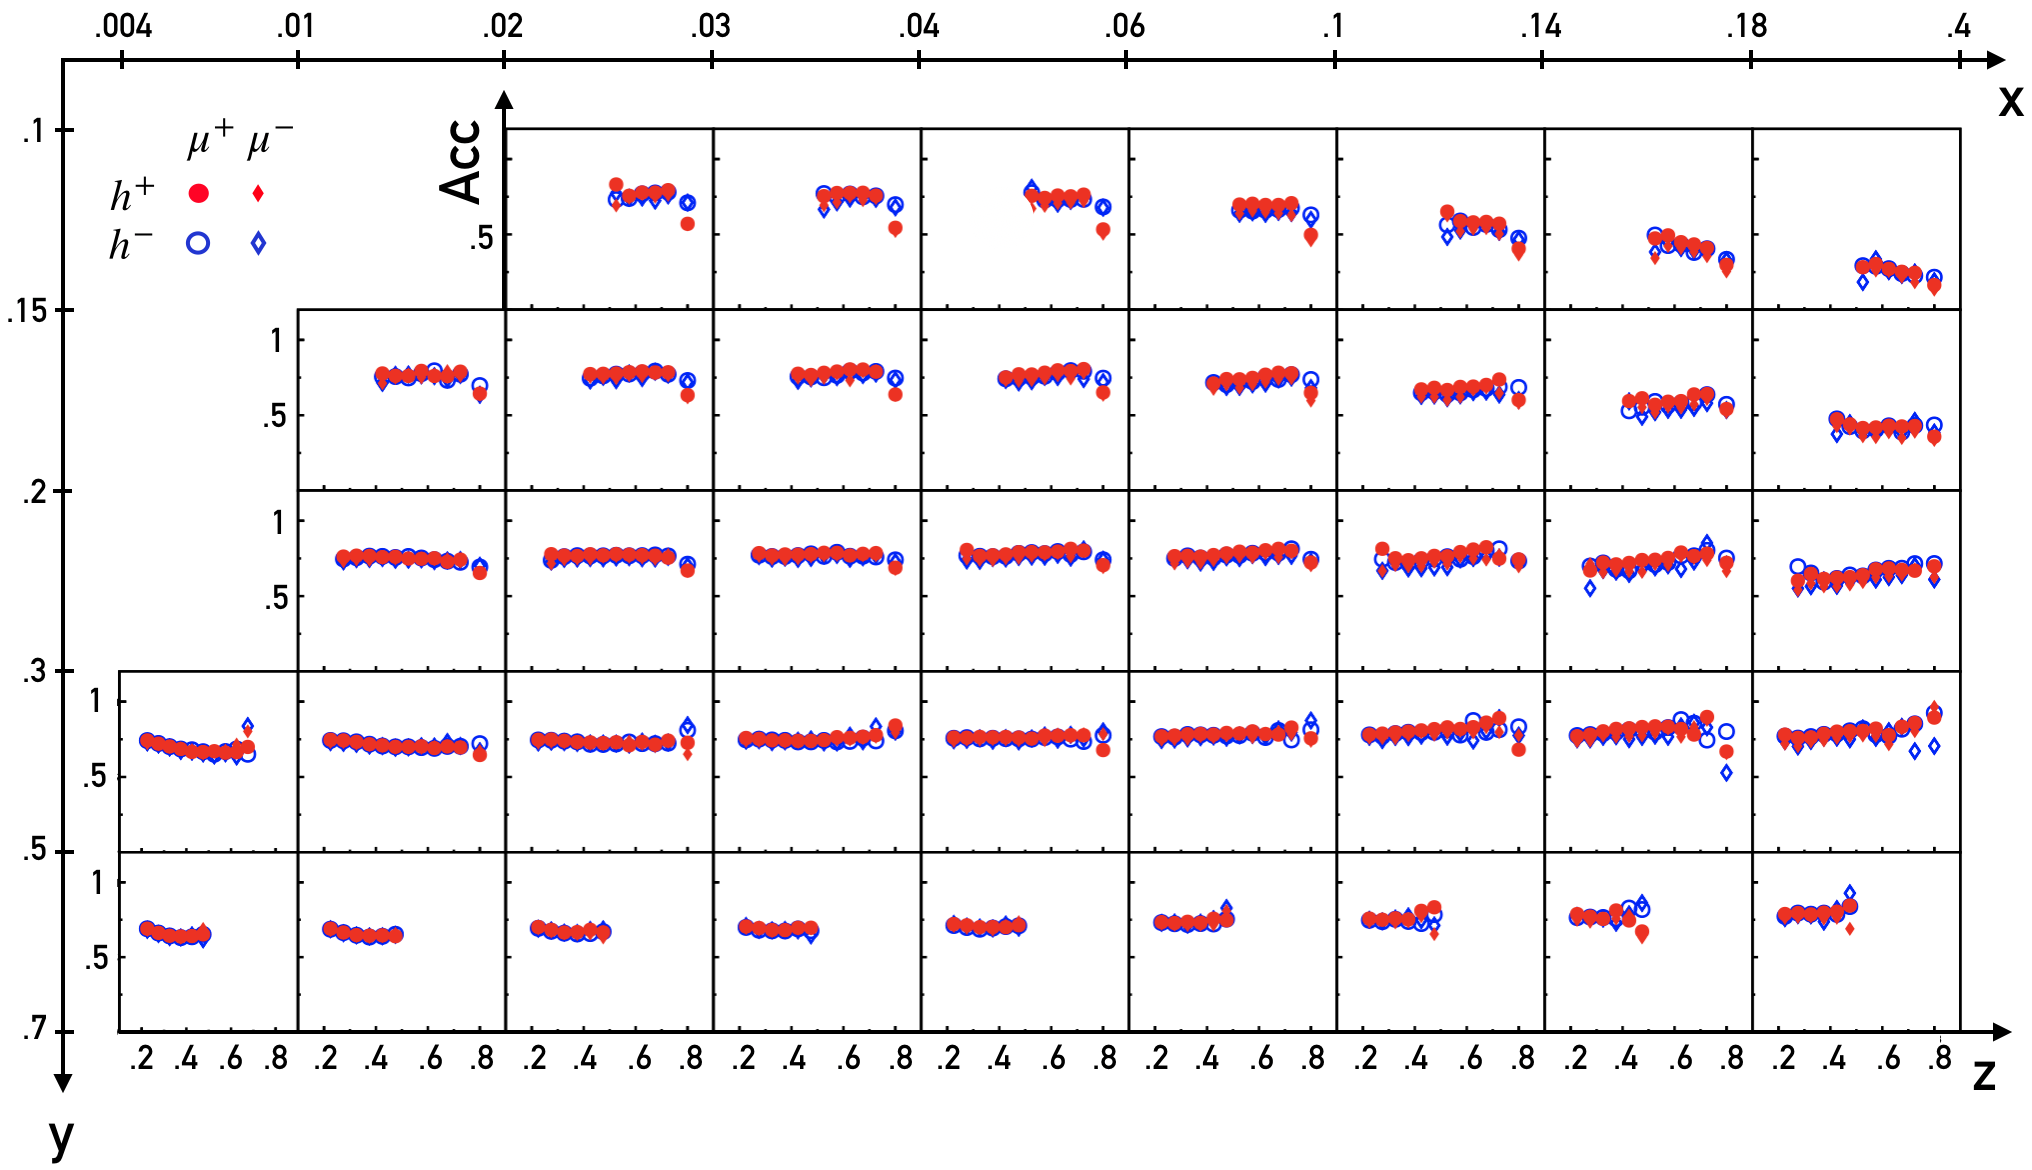
\includegraphics[scale=0.7]{./gfx/AccH.png}
	\caption{Charged hadron acceptance in $x$, $y$ and $z$ bins. The red full markers correspond to positive hadrons, blue open markers to negative hadrons, circles markers correspond to hadrons obtained with $\mu^+$ beam and diamonds markers to hadrons obtained with $\mu^-$ beam.}
	\label{pic:AccH}
\end{sidewaysfigure}

\begin{sidewaysfigure}[p]
  \centering
	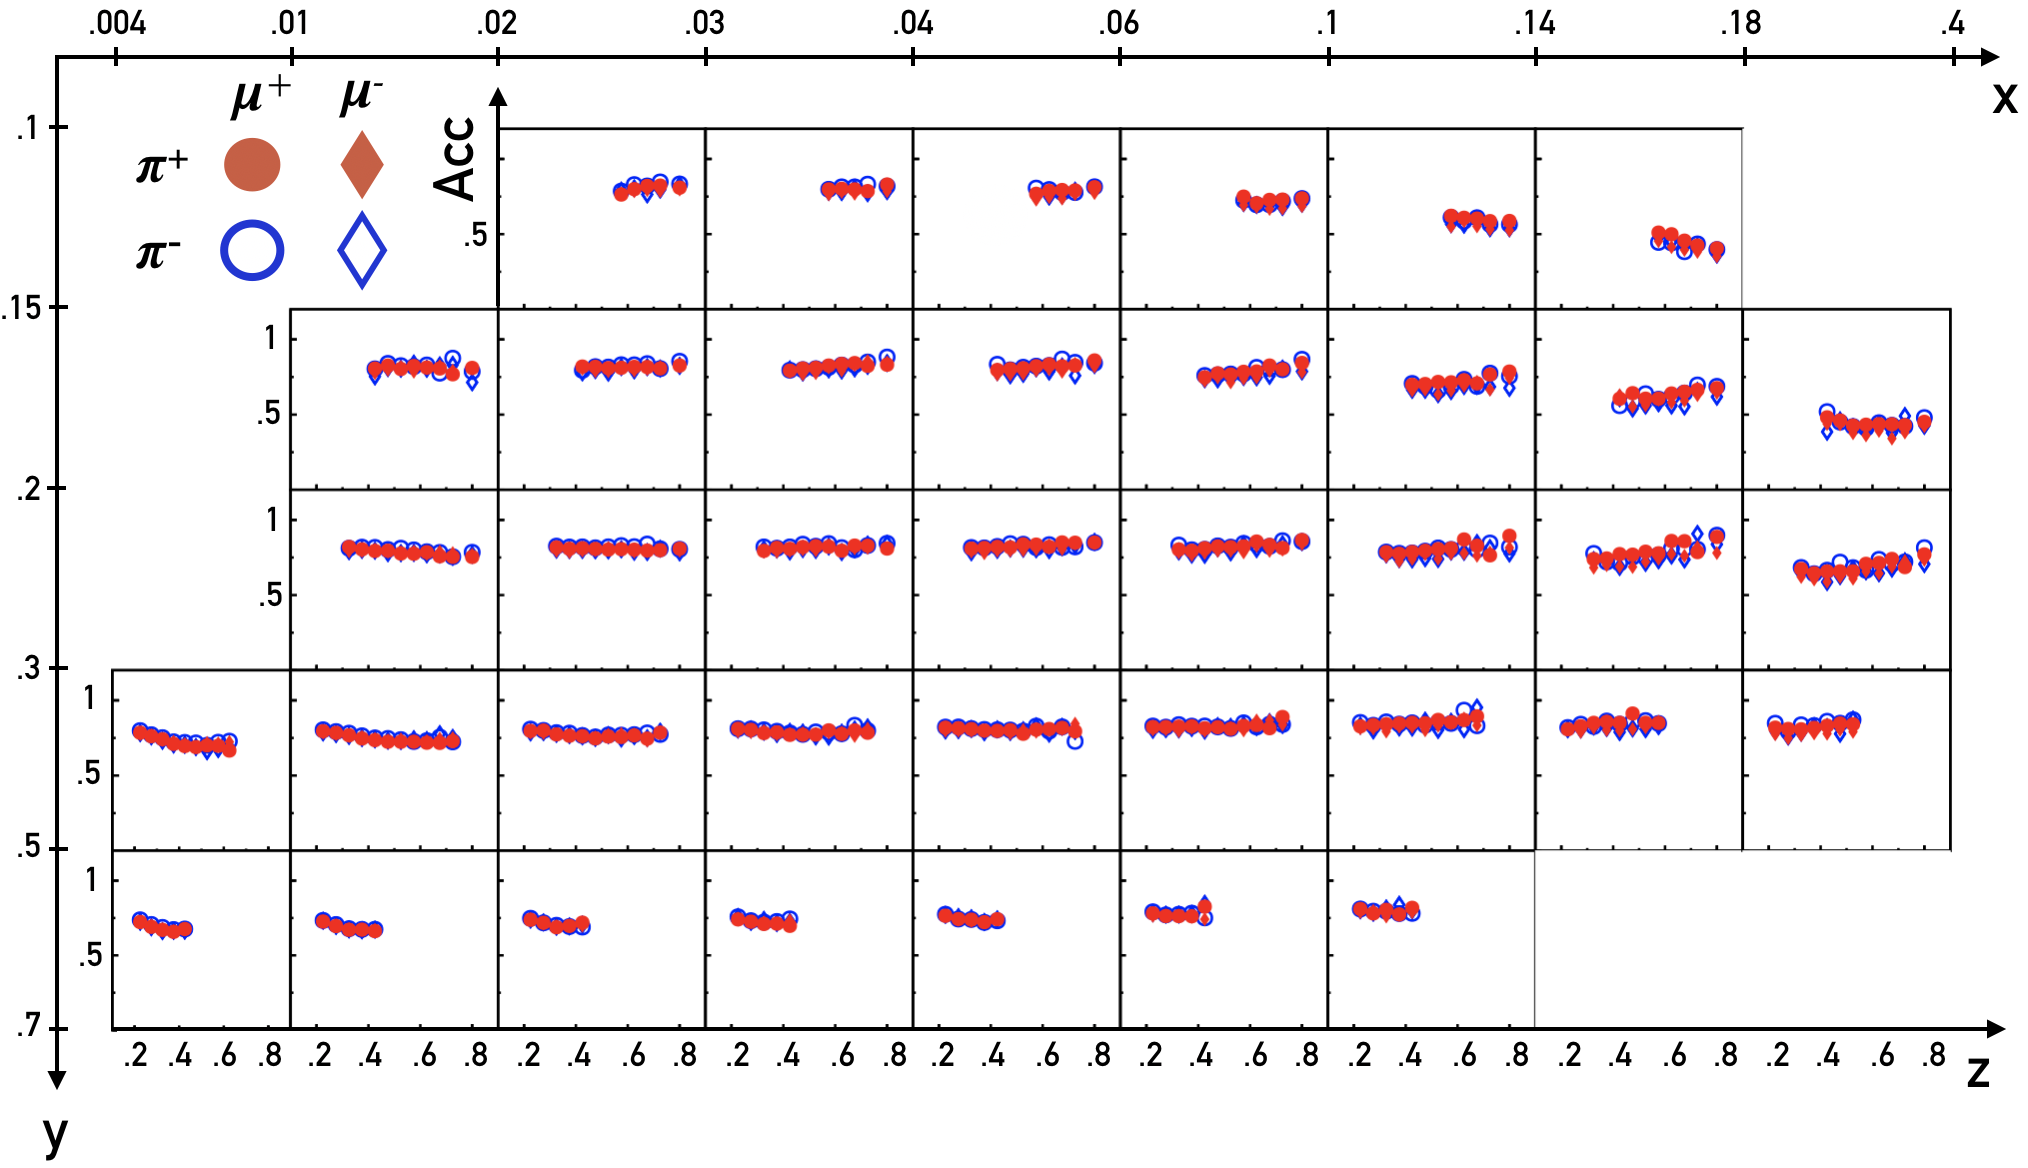
\includegraphics[scale=0.7]{./gfx/AccPi.png}
	\caption{Charged pion acceptance in $x$, $y$ and $z$ bins. The red full markers correspond to positive hadrons, blue open markers to negative hadrons, circles markers correspond to pions obtained with $\mu^+$ beam and diamonds markers to hadrons obtained with $\mu^-$ beam.}
	\label{pic:AccPi}
\end{sidewaysfigure}

\begin{sidewaysfigure}[p]
  \centering
	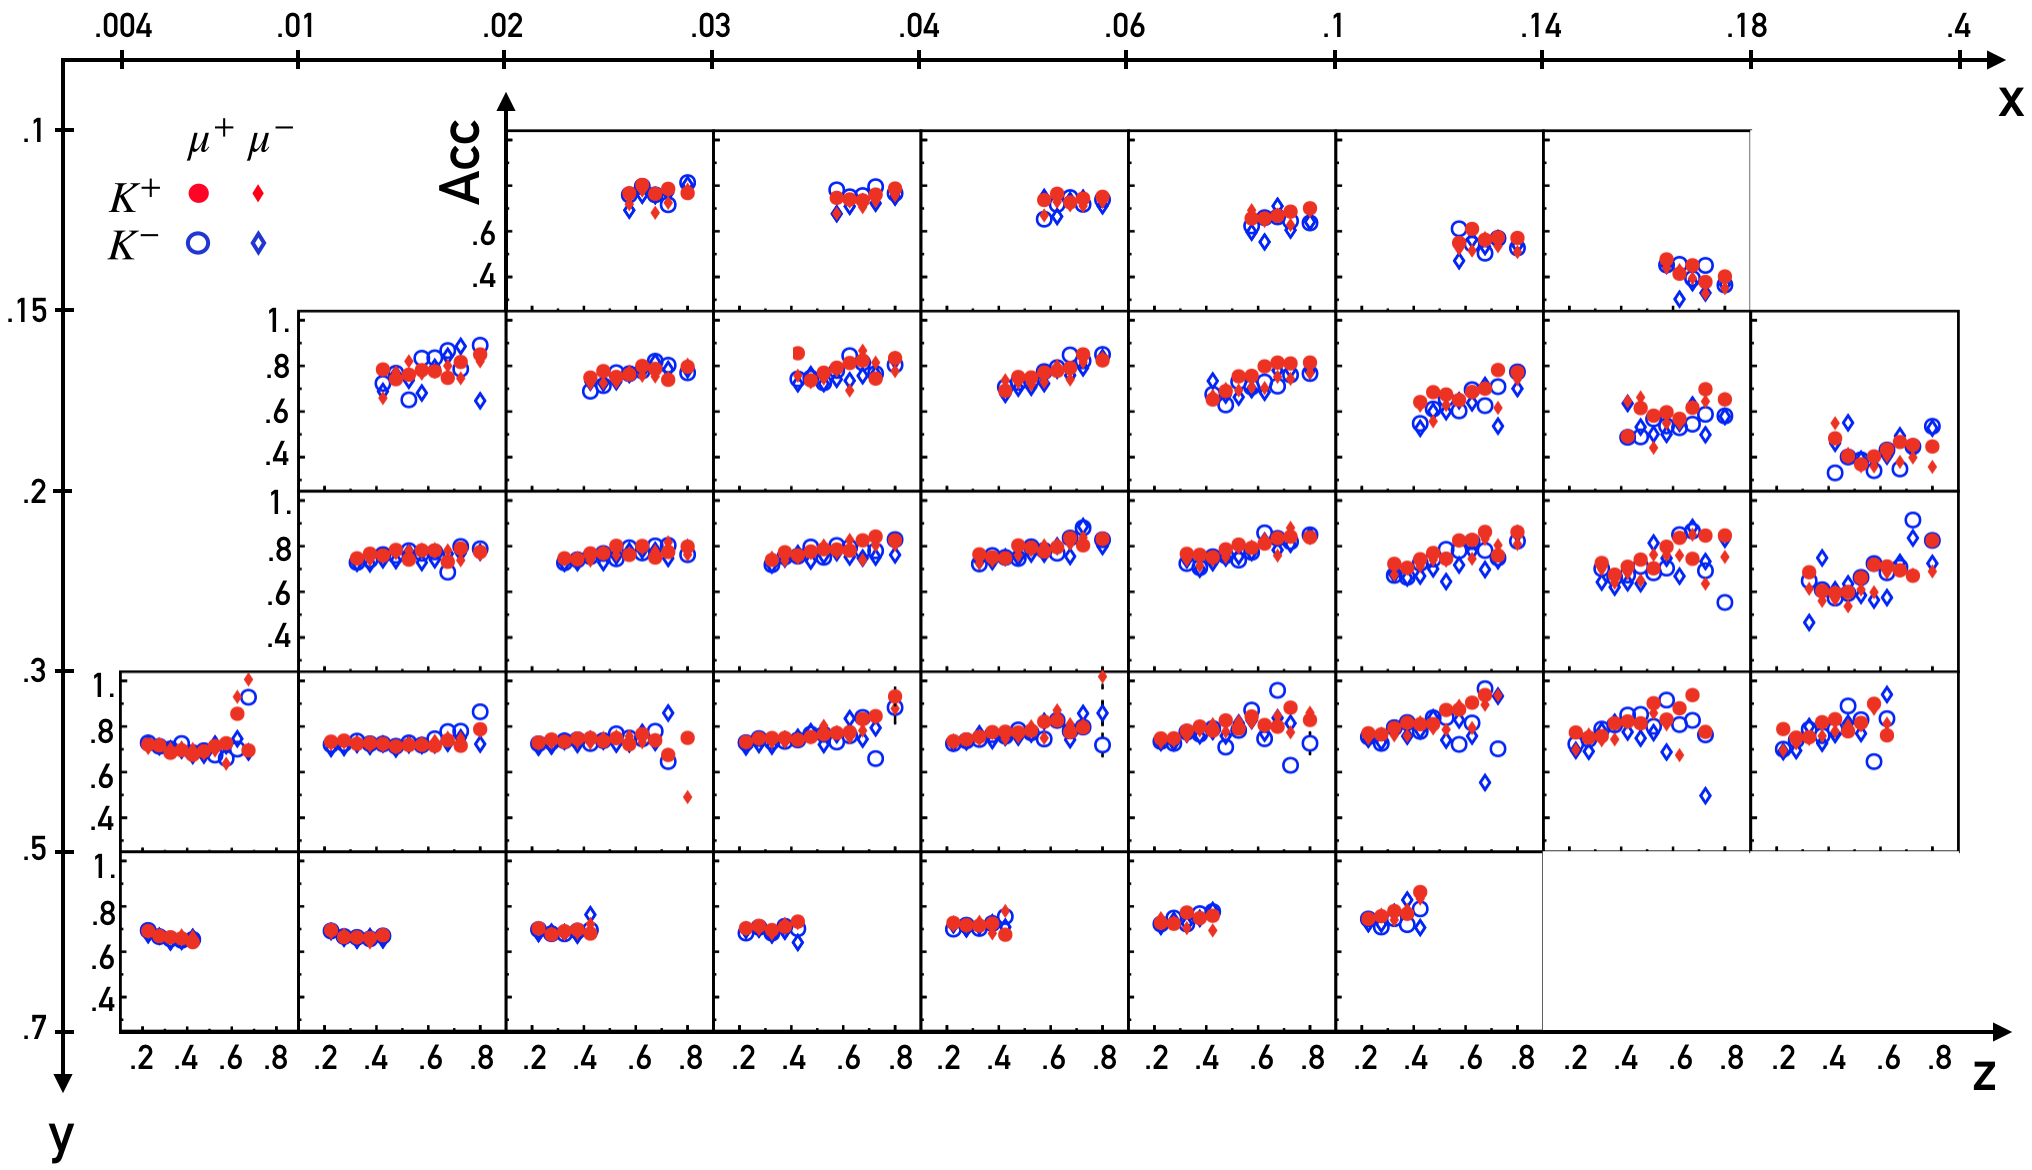
\includegraphics[scale=0.7]{./gfx/AccK.png}
	\caption{Charged kaon acceptance in $x$, $y$ and $z$ bins. The red full markers correspond to positive hadrons, blue open markers to negative hadrons, circles markers correspond to kaons obtained with $\mu^+$ beam and diamonds markers to hadrons obtained with $\mu^-$ beam.}
	\label{pic:AccK}
\end{sidewaysfigure}

\begin{sidewaysfigure}[p]
  \centering
	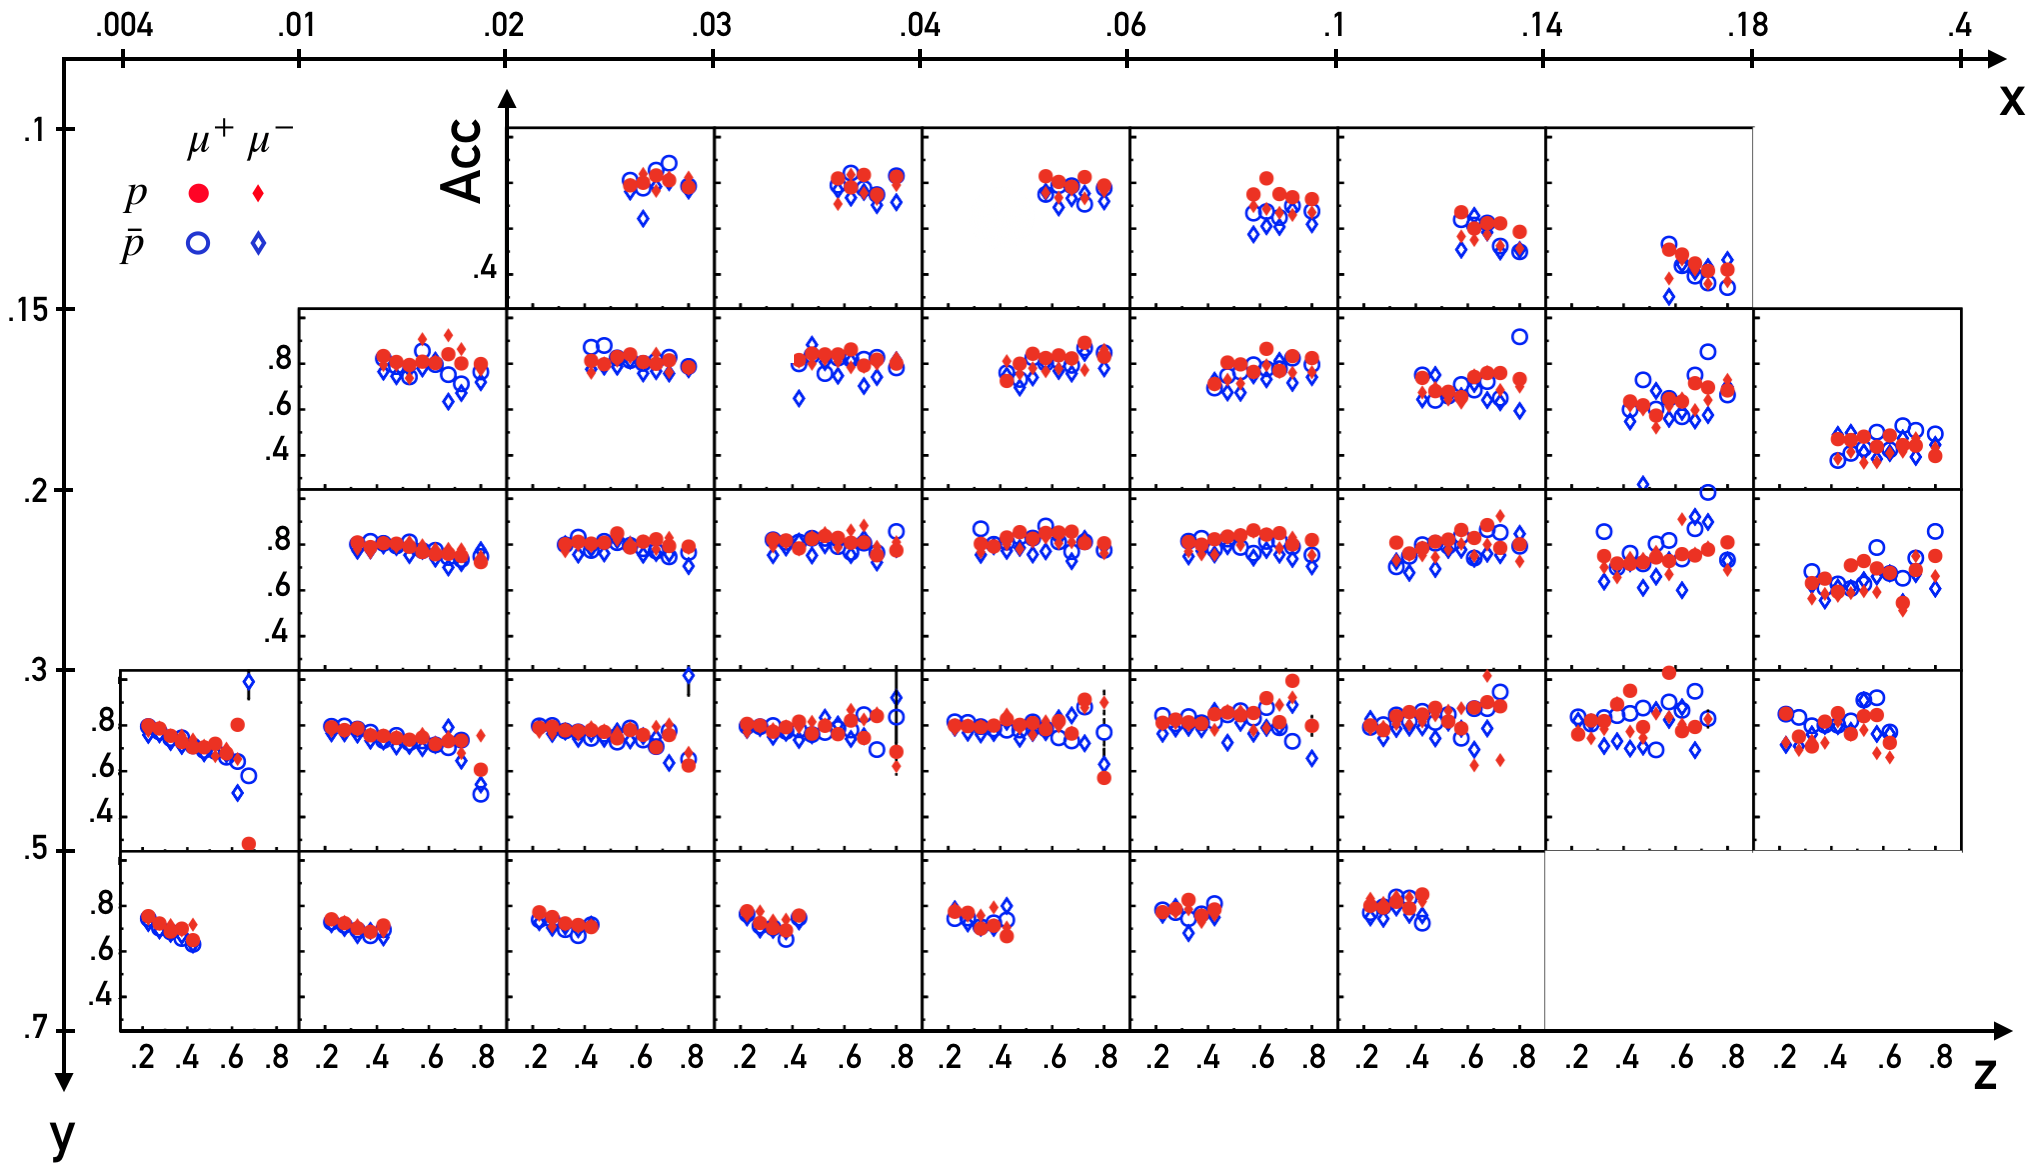
\includegraphics[scale=0.7]{./gfx/AccP.png}
	\caption{Charged proton acceptance in $x$, $y$ and $z$ bins. The red full markers correspond to positive hadrons, blue open markers to negative hadrons, circles markers correspond to kaons obtained with $\mu^+$ beam and diamonds markers to hadrons obtained with $\mu^-$ beam.}
	\label{pic:AccP}
\end{sidewaysfigure}

\begin{sidewaysfigure}[p]
  \centering
	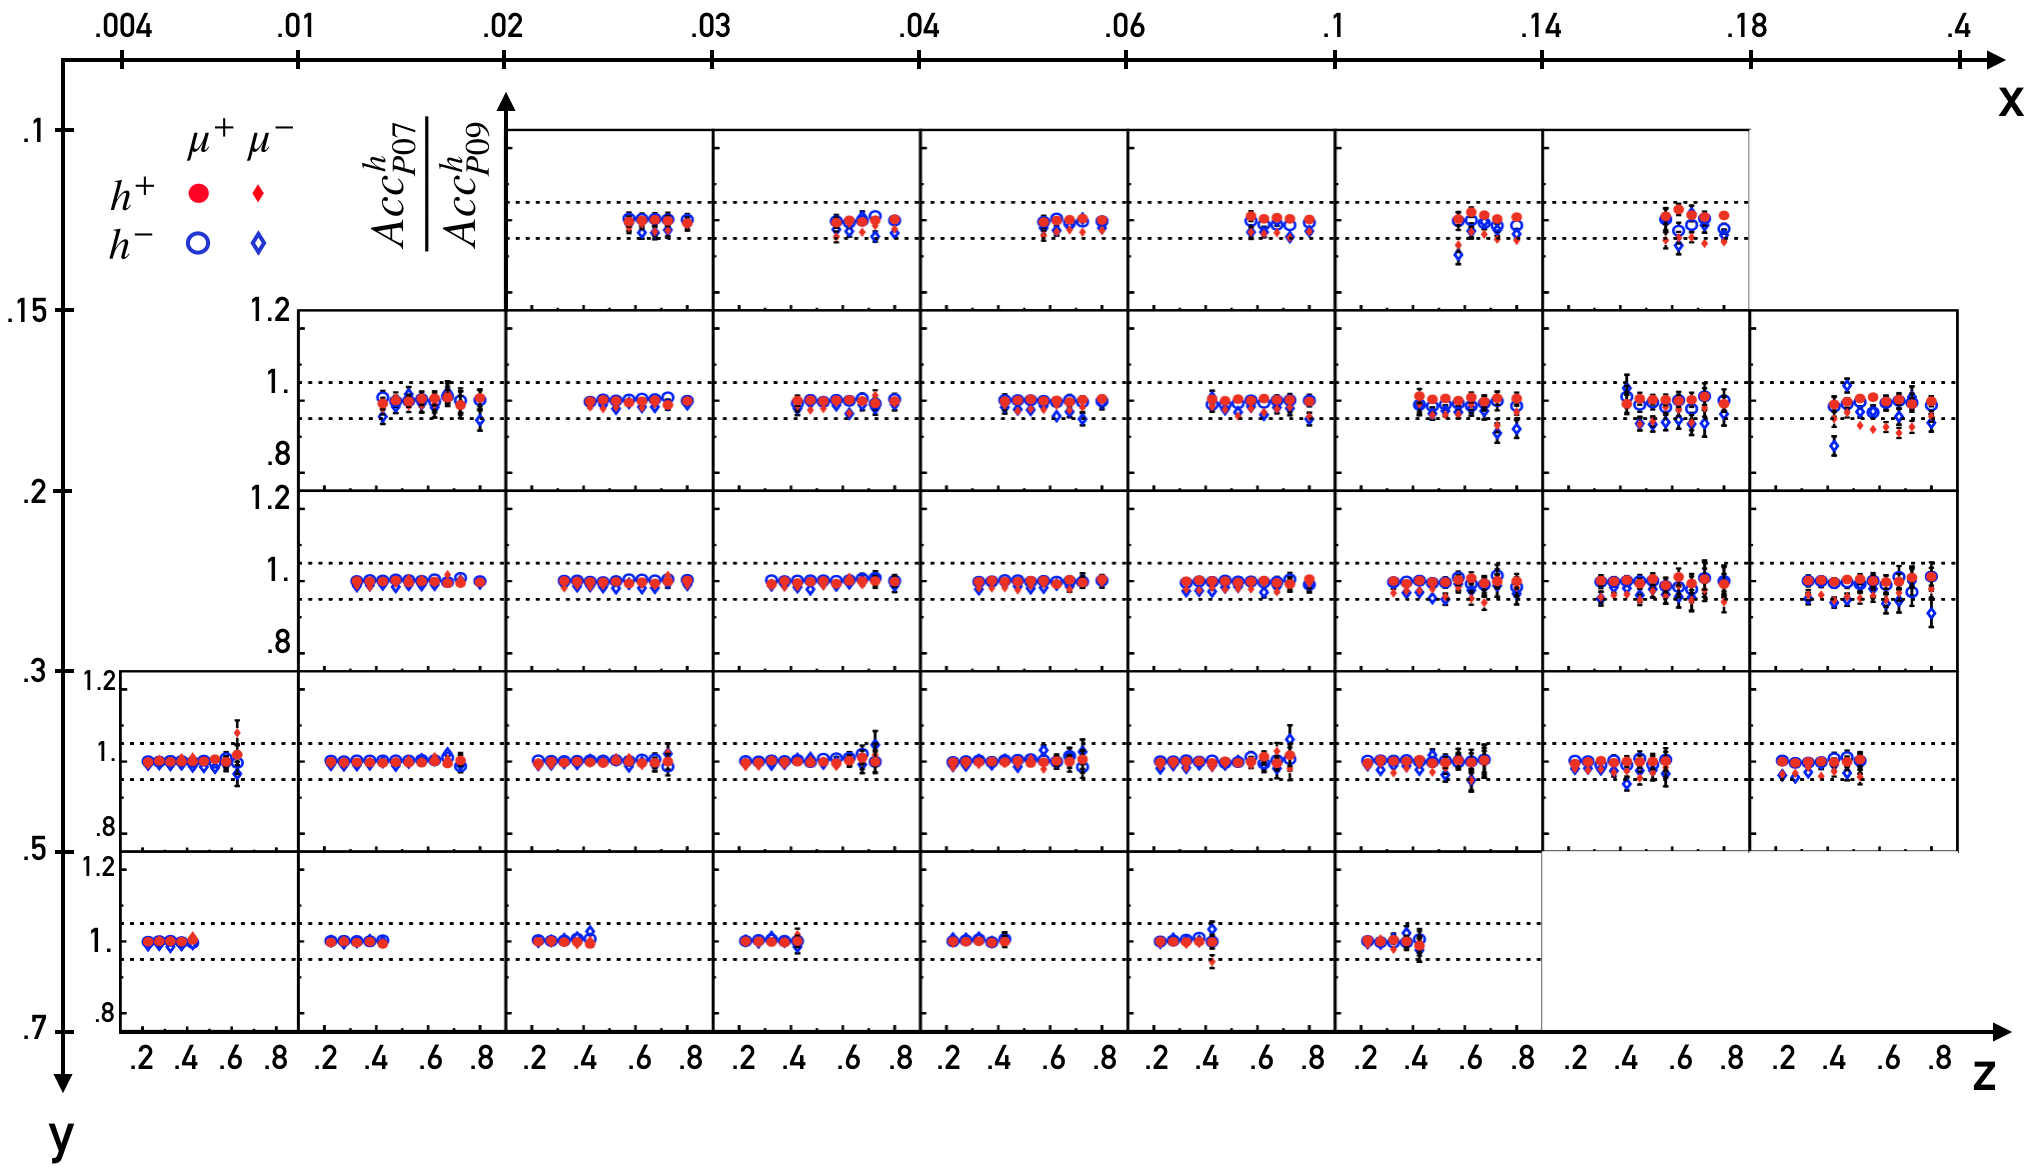
\includegraphics[scale=0.7]{./gfx/SysAcc.png}
	\caption{Ratio of P$07$ over P$09$ acceptance in $x$, $y$ and $z$ bins. The dashed lines represent a $5$\% discrepancy.}
	\label{pic:AccPer}
\end{sidewaysfigure}

In Fig.~\ref{pic:AccPer} are compared the acceptance correction factors for the P$07$ and P$09$ samples. The difference visible in the highest $x$ bins is expected and is due to the change in the trigger acceptance between P$07$ and P$08$.

The acceptance correction is then applied to the raw multiplcities:
%
\begin{equation}
  M^h(x,y,z) = \frac{M^h_{raw}(x,y,z)}{A^h(x,y,z)}
\end{equation}
%
The acceptance correction presented here was calculated with preliminary efficiencies, which should be improved in the future thus improving the correction. In addition, going back to the data over MC comparison of $theta_h$, two leads could help to improve the description. One would be to have a more detailed look at the model used inside the MC, an other would be to do acceptance in bins of $\theta_h$ but this would require more MC.

\section{Diffractive vector meson correction} \label{sec:DVMf}

It is usually assumed that hadrons produced in SIDIS originate from lepton-parton scattering. But the scattering of a lepton off a nucleon can also result in the diffractive production of vector mesons. These particles decay into lighter mesons that cannot be distinguished from the one resulting from the hadronization of a quark originating from the target nucleon. The fragmentation functions extracted from multiplicities should only come from single quark fragmentation. Thus diffractive processes should be subtracted from multiplicities.

In order to study these diffractive processes, the HEPGEN generator is used. HEPGEN \cite{HEPGEN} is a generator of Monte Carlo events, which is dedicated to studies of hard exclusive single photon or meson production processes at the COMPASS experiment kinematic domain. In addition, generation of single photon or meson production accompanied by the diffractive dissociation of the nucleon is allowed. Five processes are implemented in the generator: single photon production (DVCS+BH), exclusive $\pi^0$ production, exclusive $\rho^0$ production, exclusive $\rho^+$ production and exclusive $\Phi$ production. HEPGEN has been ported to C++ as HEPGEN++.

For pions and kaons, the dominant vector meson contribution comes from the diffractive production of $\rho^0$ and $\Phi$ (Fig.~\ref{pic:DVMprod}), respectively:
%
\begin{equation}
    \begin{split}
      \gamma * p \rightarrow \rho^0 p \rightarrow p\pi^+\pi^- \\
      \gamma * p \rightarrow \Phi p \rightarrow pK^+K^-
    \end{split}
\end{equation}
%
\begin{figure}[!h]
  \centering

  \subfloat[]{\begin{tikzpicture} \begin{feynman}
\vertex (i1) {\(l\)};
\vertex[below right=2cm of i1] (a);
\vertex[above right=2cm of a] (i2) {\(l'\)};
\vertex[below=2cm of a] (b);
\vertex[below=2cm of b] (c) {\(V\)};
\vertex[dot, below=1cm of b] (e);
\vertex[left=3cm of e] (d);
\vertex[blob, below=2cm of c] (g) {};
\vertex[above right=2cm of g] (f1) {\(\pi^+,K^+\)};
\vertex[below right=2cm of g] (f2) {\(\pi^-,K^-\)};
\vertex[above=2cm of d] (n1) {\(N\)};
\vertex[below=2cm of d] (n2) {\(N\)};


\diagram* { (i1) -- [fermion] (a) -- [fermion] (i2),
(a) -- [photon, edge label=\(\gamma^*\)] (b),
(n1) -- [double distance=7pt] (d) -- [double distance=7pt] (n2),
(n1) -- [fermion] (d) -- [fermion] (n2),
(b) -- [fermion, half left, looseness=1.5, edge label=\(q\)] (c),
(b) -- [anti fermion, half right, looseness=1.5, edge label=\(\bar{q}\)] (c),
(d)-- [plain, half left, looseness=1.5] (e),
(d)-- [plain, half right, looseness=1.5] (e),
(c) -- [double distance=7pt] (g) [blob],
(g) [blob] -- [double distance=7pt] (f1),
(g) [blob] -- [double distance=7pt] (f2),
};
\end{feynman} \end{tikzpicture}}
\hspace{2cm}
\subfloat[]{\begin{tikzpicture} \begin{feynman}
\vertex (i1) {\(l\)};
\vertex[below right=2cm of i1] (a);
\vertex[above right=2cm of a] (i2) {\(l'\)};
\vertex[dot, below=2cm of a] (b);
\vertex[below=2cm of b] (c) {\(V\)};
\vertex[below=1cm of b] (e);
\vertex[left=3cm of e] (d);
\vertex[blob, below=2cm of c] (g) {};
\vertex[above right=2cm of g] (f1) {\(\pi^+,K^+\)};
\vertex[below right=2cm of g] (f2) {\(\pi^-,K^-\)};
\vertex[above=2cm of d] (n1) {\(N\)};
\vertex[below=2cm of d] (n2) {\(X\)};


\diagram* { (i1) -- [fermion] (a) -- [fermion] (i2),
(a) -- [photon, edge label=\(\gamma^*\)] (b),
(n1) -- [double distance=7pt] (d) -- [double distance=7pt] (n2),
(n1) -- [fermion] (d) -- [plain] (n2),
(b) -- [fermion, half left, looseness=1.5, edge label=\(q\)] (c),
(b) -- [anti fermion, half right, looseness=1.5, edge label=\(\bar{q}\)] (c),
(d) -- [plain, half left, looseness=1.5] (e),
(d) -- [plain, half right, looseness=1.5] (e),
(c) -- [double distance=7pt] (g) [blob],
(g) [blob] -- [double distance=7pt] (f1),
(g) [blob] -- [double distance=7pt] (f2),
};
\end{feynman} \end{tikzpicture}}
	\caption{Vector meson diffractive production (V in the figure, being $\rho^0$, $\Phi$, etc..). In the VMD model \cite{VMD}, the $\gamma^*$ virtual photon creates a $q\bar{q}$ pair with compatible quantum numbers. Two cases can be encountered: vector meson exclusive production (where the same nucleon is found in the final state) (a) and vector meson production with nucleon diffractive dissociation (b).}
	\label{pic:DVMprod}
\end{figure}

This process is mainly exclusive but in $20$\% of cases a diffractive dissociation of the target nucleon occurs. Other channels (excited $\rho$, $\omega$, etc.) are expected to contribute much less and are not taken into account. As pions and kaons stemming from diffractive vector meson decay cannot be separated from the one resulting from SIDIS, the evaluation of their contribution to the multiplicities is based on a Monte Carlo study. Three Monte Carlo samples are produced based on different generators (SIDIS using DJANGOH, diffractive $\Phi$ and $\rho^0$ using HEPGEN++). All this samples are reconstructed with the same event reconstruction chain as data. For the diffractive vector meson samples, both exclusive events and events with diffractive dissociation of the proton are simulated.

The fraction of pions (resp. kaons) resulting from a diffractive $\rho^0$ (resp. $\Phi$) is calculated in the same binning as the raw multiplicities as:
%
\begin{equation}\label{eq:DVMhad}
  \begin{split}
    f^{\pi}_{\rho^0}(x,y,z) = \frac{N^{\pi}_{HEPGEN++}(x,y,z)}{N^{\pi}_{DJANGOH}(x,y,z)+N^{\pi}_{HEPGEN++}(x,y,z)} \\
    f^K_{\Phi}(x,y,z) = \frac{N^K_{HEPGEN++}(x,y,z)}{N^K_{DJANGOH}(x,y,z)+N^K_{HEPGEN++}(x,y,z)}
  \end{split}
\end{equation}
%
where $N^{\pi}_{HEPGEN++}$, $N^{\pi}_{DJANGOH}$, $N^K_{HEPGEN++}$ and $N^K_{DJANGOH}$ are the number of kaons reconstructed from the HEPGEN++ and DJANGOH MC samples normalized by the corresponding MC luminosity ($L_{MC}$). The luminosity depends on the event weighting and the process cross-section $\sigma_{int}$ (DIS for DJANGOH event and diffractive vector meson production for HEPGEN++ events):
%
\begin{equation} \label{eq:reweight}
  \sum_{events} w_i = L_{MC} \cdot \sigma{int}.
\end{equation}
%
The final weighted number of DIS events and hadrons is summarized in Table~\ref{DVM}.

\begin{table}
	\centering
	\begin{tabular}{rccc}
    \hline
     & DJANGOH & $\rho^0$ & $\Phi$ \\
    \hline
    Generated Events & 8.4M & 19.1M & 19.2M  \\
    Weighted Generated Events & 8.4M & 280.2M & 576.9M  \\
		Integrated Cross-Section [pb] & 227010 & 12200 & 2500  \\
		Monte-Carlo Luminosity [pb$^-1$] & 36.8 & 22966.6 & 23075.2  \\
    \hline
		DIS Events [pb] & 3.4M & 96209 & 18083  \\
		$h^+$ [pb] & 630880 & 25301 & 3890  \\
		$h^-$ [pb] & 511014 & 25250 & 4033  \\
		$\pi^+$ [pb] & 453794 & 25257 & -  \\
		$\pi^-$ [pb] & 377335 & 25212 & -  \\
		$K^+$ [pb] & 102019 & - & 3872  \\
		$K^-$ [pb] & 75158 & - & 4015 \\
  \end{tabular}
  \caption{Weighted number of DIS events and hadrons for the diffractive vector meson correction.}
  \label{DVM}
\end{table}

The same MC samples are also used to determine diffractive vector meson contribution to the DIS sample. The diffractive vector meson events can also lead to a contamination in DIS events. Here, the two channels studied are diffractive $\rho^0$ and $\Phi$ with the fraction of the contamination expressed in Eq.~\ref{eq:DVMDIS}.

\begin{sidewaysfigure}[!]
  \centering
	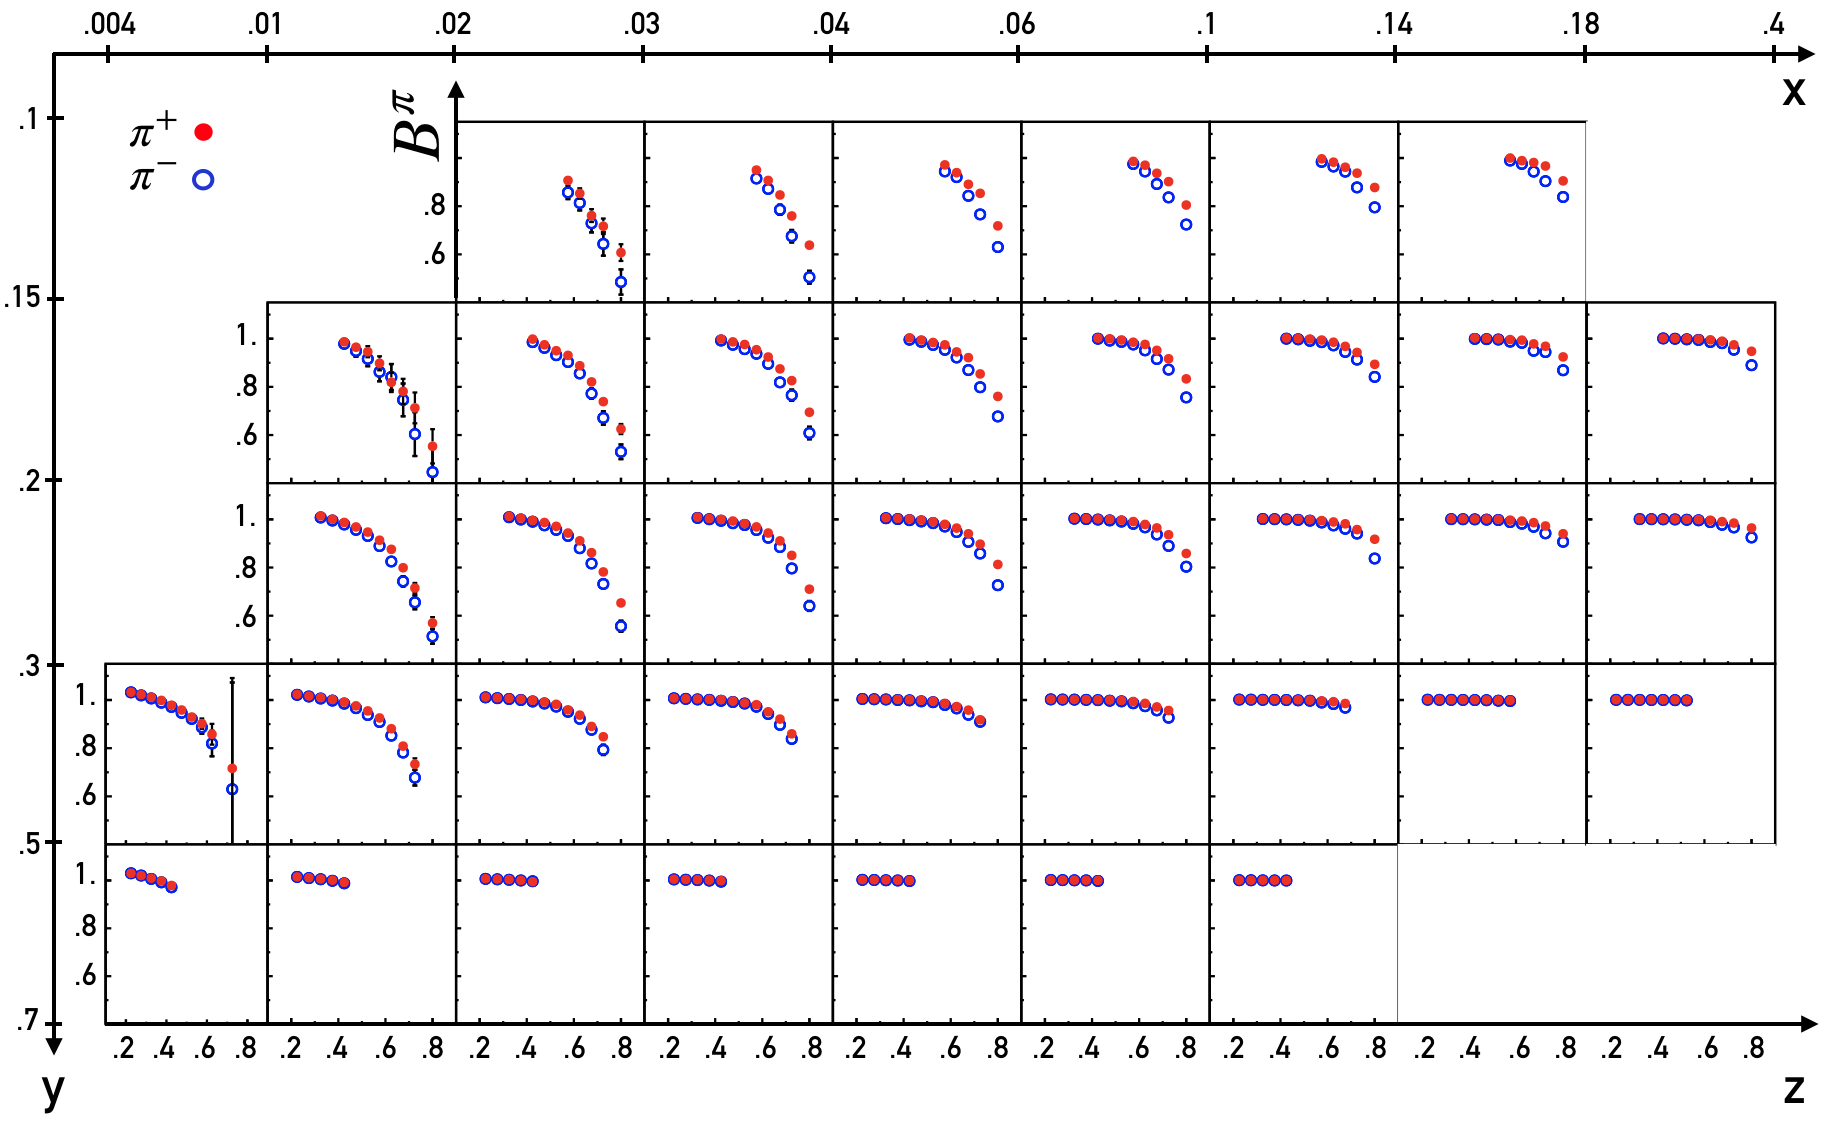
\includegraphics[scale=0.8]{./gfx/DVMpi.png}
	\caption{Correction factor $B^{\pi}$ for diffractive vector meson contamination ($\rho^0$) as a function of $z$ for ($x$,$y$) bins. The red markers correspond to positive pions and blue markers for negative pions.}
	\label{DVMpi}
\end{sidewaysfigure}

\begin{sidewaysfigure}[!]
  \centering
	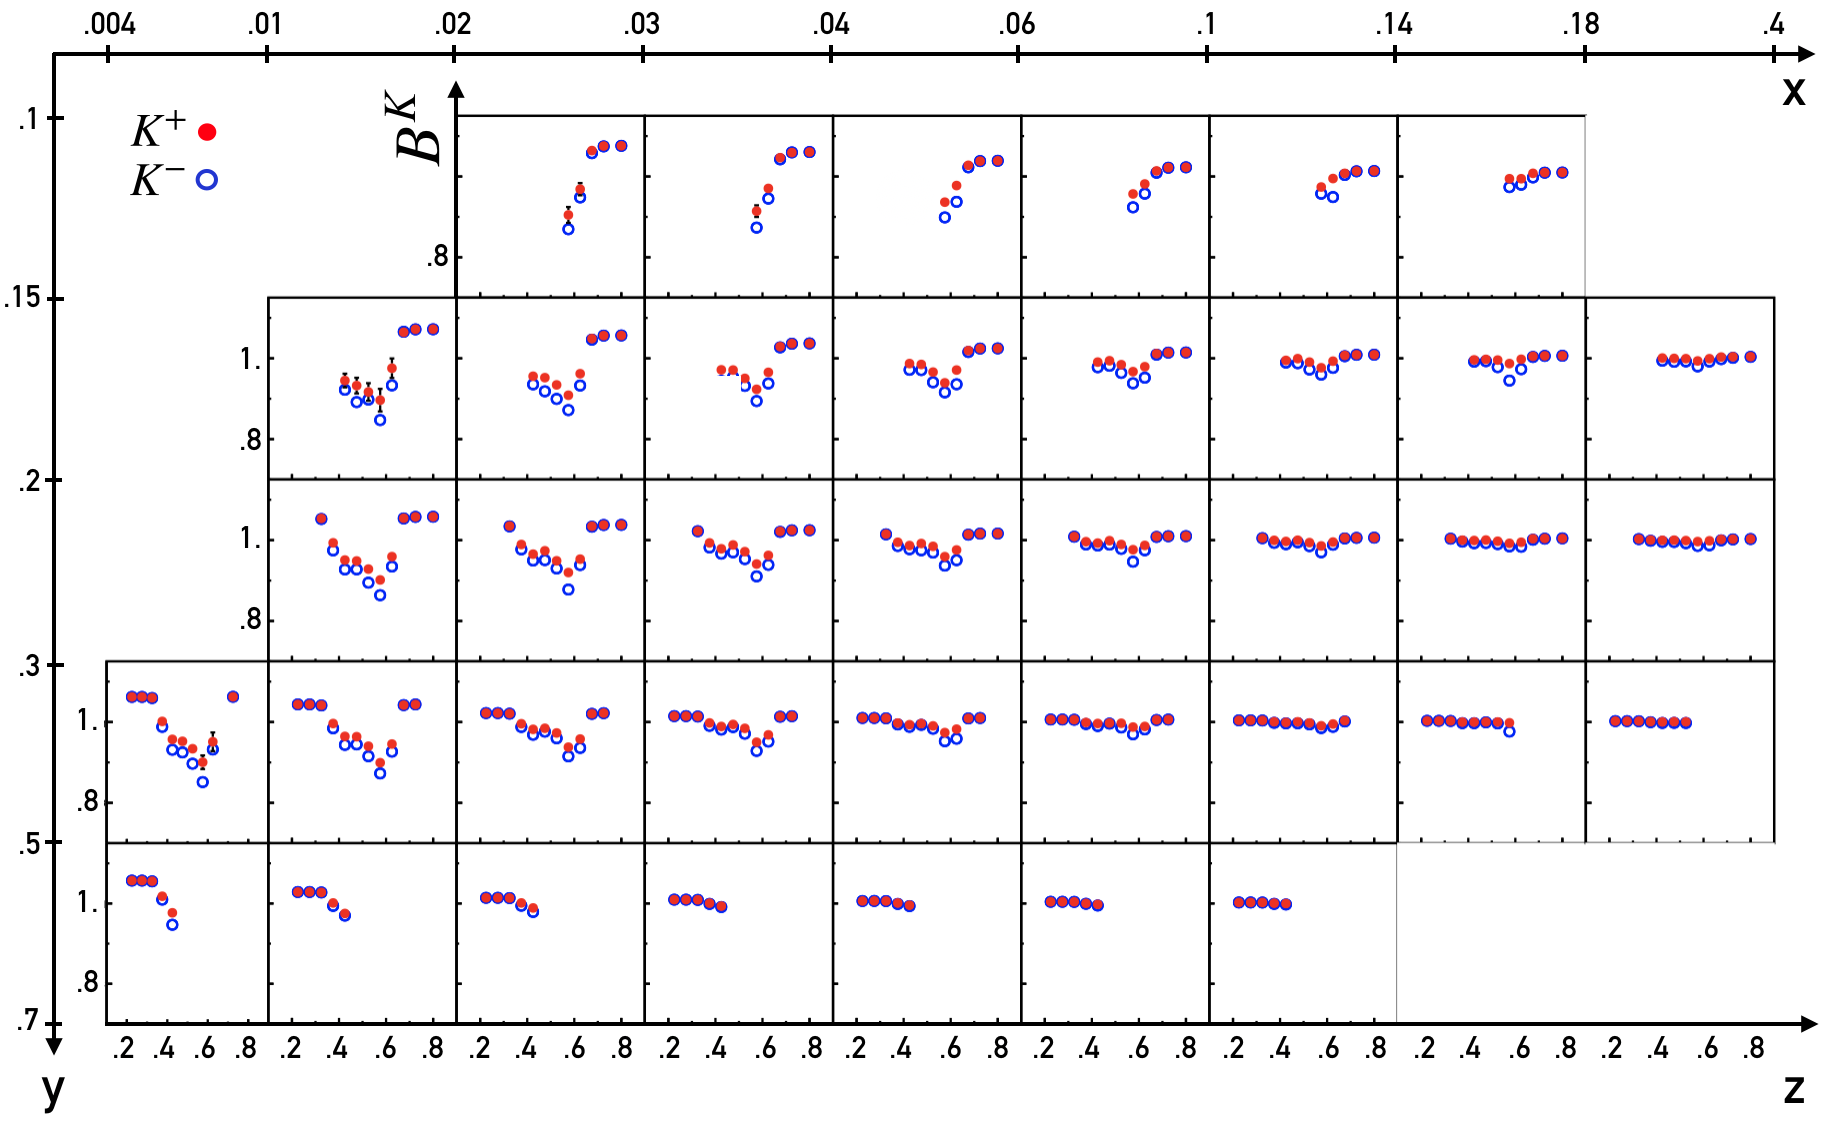
\includegraphics[scale=0.8]{./gfx/DVMK.png}
	\caption{Correction factor $B^{K}$ for diffractive vector meson contamination ($\Phi$) as a function of $z$ for ($x$,$y$) bins. The red markers correspond to positive kaons and blue markers for negative kaons.}
	\label{DVMK}
\end{sidewaysfigure}
%
\begin{equation}\label{eq:DVMDIS}
  \begin{split}
    f^{\rho^0}_{DIS}(x,y,z) = \frac{N^{DIS}_{\rho^0,HEPGEN++}(x,y,z)}{N^{DIS}_{DJANGOH}(x,y,z)+N^{DIS}_{\rho^0,HEPGEN++}(x,y,z)+N^{DIS}_{\Phi,HEPGEN++}(x,y,z)} \\
    f^{\Phi}_{DIS}(x,y,z) = \frac{N^{DIS}_{\Phi,HEPGEN++}(x,y,z)}{N^{DIS}_{DJANGOH}(x,y,z)+N^{DIS}_{\rho^0,HEPGEN++}(x,y,z)+N^{DIS}_{\Phi,HEPGEN++}(x,y,z)}
  \end{split}
\end{equation}
%
The total contribution from the diffractive vector-meson contribution to the DIS sample is $f^{VM}_{DIS} = f^{\rho^0}_{DIS} + f^{\Phi}_{DIS}$. The final correction reads as follows:
%
\begin{equation}
  \begin{split}
  B^h(x,y,z) = \frac{ \frac{N^{\pi}(x,y,z)}{N^h(x,y,z)}\left (1-f^{\pi}_{\rho^0}(x,y,z)\right )
                   + \frac{N^K(x,y,z)}{N^h(x,y,z)}\left (1-f^{K}_{\Phi}(x,y,z)\right ) + \frac{N^p(x,y,z)}{N^h(x,y,z)} }{1-f^{VM}_{DIS}(x,y,z)} \\
  B^{\pi}(x,y,z) = \frac{1-f^{\pi}_{\rho^0}(x,y,z)}{1-f^{VM}_{DIS}(x,y,z)} \\
  B^K(x,y,z) = \frac{1-f^{K}_{\Phi}(x,y,z)}{1-f^{VM}_{DIS}(x,y,z)}.
  \end{split}
\end{equation}
%
and are displayed in Fig.~\ref{DVMpi} for the correction for pions and in Fig.~\ref{DVMK} for the correction for kaons. The correction for pions has the strongest impact at high $z$ ($z>0.5$) and low $x$ ($x<0.02$) where it can reach $50$\%, while the correction for kaons has the strongest impact at middle $z$ ($0.4<z<0.6$) and low $x$ ($x<0.02$), where it can reach $20$\%.

\section{Radiative corrections} \label{sec:rcf}

The experimental multiplicities are affected by QED radiative effects, which introduce a systematic bias of the measured kinematics with respect to the true kinematics. The correction factor taking into account these contributions is the radiative correction factor defined as:

\begin{equation}
	\eta(x,y,z) = \frac{d^2 M_{1\gamma}/dxdydz}{d^2 M_{measured}/dxdydz}
\end{equation}

where $M_{1\gamma}$ denotes multiplicities obtained using the cross-section in the one photon exchange approximation and $M_{measured}$ denotes multiplicities obtained using the measured cross-section which includes radiative effects. The bias on the $\mu$ kinematics upon real photon emission affects in turn the reconstruction of the kinematic variables $x$, $y$ and $z$. This effect is now taken into account thanks to DJANGOH. Previously in this chapter, DJANGOH was used as an event generator for our Monte Carlo simulation but it can also be used to compute radiative corrections. At generator level, one sample of multiplicities with radiative corrections and one without are generated and from these two samples $\eta(x,y,z)$ is calculated. Fig.~\ref{fig:hadz_ratio} in Chapter~\ref{ch:RC}, Section~\ref{sec:RCFMult} shows the effect of the correction. A statistical error is associated to this correction due to the non-analytical nature of the calculation. Obtaining the radiative correction in bins of ($x,y,z$) is a novelty in COMPASS.

\section{Electron contamination}

The pion (and thus hadron) sample is contaminated by electrons and positrons. With the DJANGOH event generator, we are able to describe almost correctly the electron production from radiative photons: in Fig.~\ref{pic:Eprod2016} one can see that the discrepancy of electroproduction in $\Phi$ in the hadron production plane is up to $10$\% at low $\Phi$. Given the overall small size of the correction it was decided to use the MC sample for corrections at momenta, where the electron identification cannot be provided by the RICH detector. The fraction of electrons in the pion samples obtained in the range $12$ $< p_h <$ $40$ GeV in the MC sample is shown in Fig.~\ref{pic:epi}. This contamination goes from $5$\% at low $z$ to $1$\% at high $z$. The correction is taken into account in the acceptance correction, taking the electrons in the reconstructed sample (as in data) and not in the generated one. The correction looks reasonable and further scrutinizing of this analysis is on the way.

\begin{sidewaysfigure}[!p]
	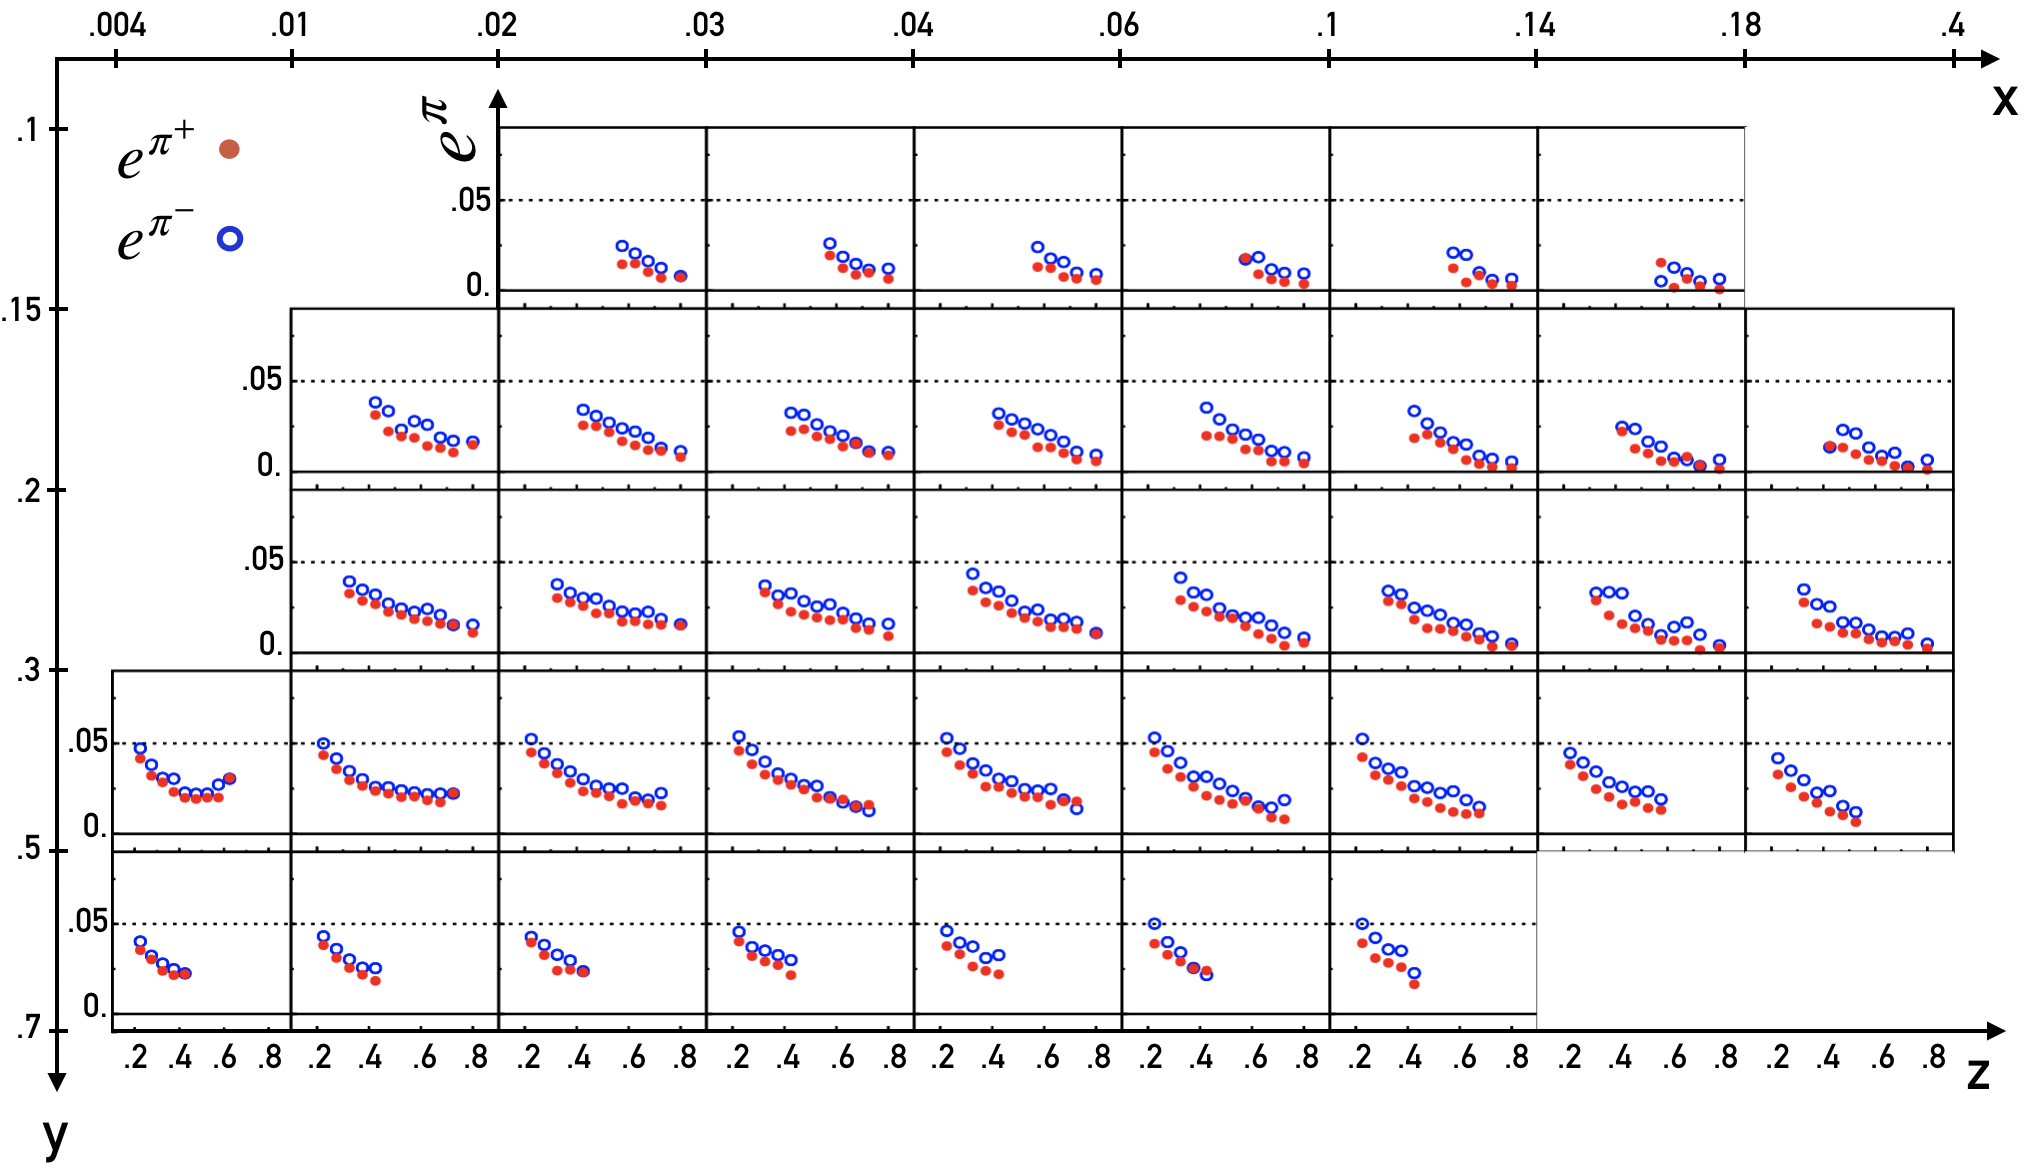
\includegraphics[scale=0.7]{./gfx/econt.png}
	\caption{Fraction of electron contamination for pions as a function of $z$ in bins of $x$ (columns) and $y$ (rows). Red markers are for $\pi^+$ and blue markers for $\pi^-$.}
	\label{pic:epi}
\end{sidewaysfigure}

\section{Summary}

The most important correction is the acceptance $A(x,y,z)$, which accounts for the geometrical limitations of the apparatus, the data reconstruction efficiency and the detector efficiencies. This correction for charged hadrons is mostly of $70$\% but can drop down to $30$\% in some bins. The electron contamination correction, which corrects for the inability of the RICH to distinguish electrons and pions above $8$ GeV/$c$, is embedded inside the acceptance correction.

The correction factor for the vector meson production $B^h(x,y,z)$ contaminating the hadron sample varies from $0$ to $40$\% at high $z$ for pions and $0$ to $20$\% at medium $z$ for kaons. As these cross-sections are experimentally not known, model calculations are to evaluate this correction.

The correction factor related to the radiative corrections, taking into account the change of hadron and lepton kinematic variables due to the emission of a real photon, hence biaising the kinematic distributions, is going from $0$ to $20$\%, the highest correction being located at high $y$, high $z$ and low $x$.
